\documentclass{article}
\usepackage[utf8]{inputenc}
\usepackage[brazil]{babel}
\usepackage[a4paper, top=2.5cm, bottom=2.5cm, left=2cm, right=2.5cm]{geometry}
\usepackage{makecell}

\usepackage{graphicx}
\graphicspath{{figures/}}

% PB: redefinir maketitle
\makeatletter
\def\@maketitle
{
    \begin{flushleft}
        \let \footnote \thanks
        {\Large \textbf{\@title} \par}
        \vskip 1em
        {\large \textbf{\@author} \par}
        \vskip 1em
        {\large \textit{\@date}}
    \end{flushleft}
    \par
    \vskip 1.5em
}
\makeatother

\title{Aprendizado por Reforço}
\author{Aula 01 - Introdução ao Aprendizado por Reforço}
\date{Paulo Bruno de Sousa Serafim - Outubro 2019}

\begin{document}

\maketitle

\section{O que é ``reforço''}

    \subsection{Condicionamento}
    
        \subsubsection{Condicionamento Clássico}
        
            Reação \textbf{involuntária} a um estímulo treinado.
        
        \subsubsection{Condicionamento Operante}
        
            Açao \textbf{voluntária} para obter uma resposta desejável.
        
    \subsection{Reforço vs. Punição}
    
        \subsubsection{Reforço}
        
            \begin{itemize}
                \item Processo em que a ocorrência de um comportamento é fortalecida por uma consequência de sua ocorrência;
                \item Aumenta a frequência do comportamento.
            \end{itemize}
        
        \subsubsection{Punição}
        
            \begin{itemize}
                \item Processo em que a ocorrência de um comportamento é enfraquecida por uma consequência de sua ocorrência;
                \item Diminui a frequência do comportamento.
            \end{itemize}
            
        \subsubsection{Positivo}
        
            \begin{itemize}
                \item Relacionado ao acréscimo ou adição de algo.
            \end{itemize}
        
        \subsubsection{Negativo}

            \begin{itemize}
                \item Relacionado à ausência ou subtração de algo.
            \end{itemize}
        
        \begin{table}[ht]
            \centering
            \begin{tabular}{|c|c|c|}
                \hline
                 & \textbf{Adiciona estímulo} & \textbf{Remove ou evita estímulo} \\
                \hline
                \makecell{\textbf{Aumenta a chance de ocorrência} \\ \textbf{do comportamento}} & Reforço Positivo & Reforço Negativo \\ 
                \hline
                \makecell{\textbf{Diminui a chance de ocorrência} \\ \textbf{do comportamento}} & Punição Positiva & Punição Negativa \\ 
                \hline
            \end{tabular}
            \caption{Relação entre estímulo e chance de ocorrência de um comportamento}
            \label{tab:reforco-punicao}
        \end{table}
        
        \begin{figure}[ht]
            \centering
            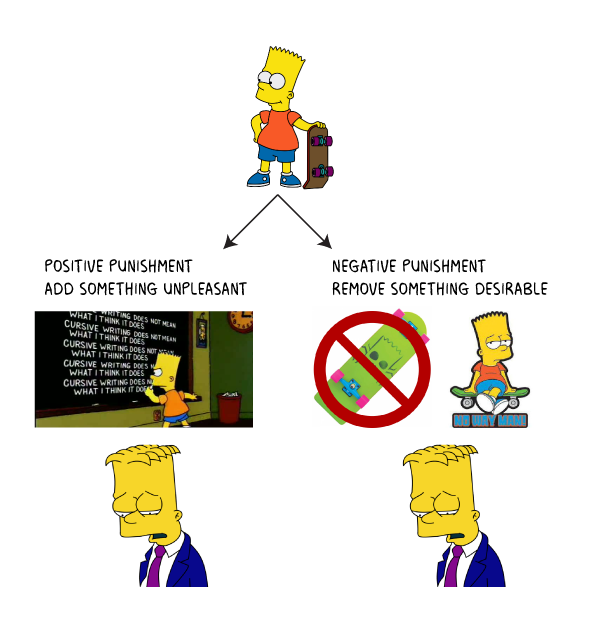
\includegraphics[width=250pt]{bart-punishment.png}
            \caption{Fonte: Shrestha (2017)}
            \label{fig:bart-punicao}
        \end{figure}
        
\section{Exemplos}

    \begin{itemize}
        \item Cachorro que toca campainha para receber petisco;
        \item Criança que pega na tomada;
        \item Jogador que aprende a jogar algum jogo.
    \end{itemize}
        
\section{Características}

    \begin{itemize}
        \item Aprendizado através da interação com o ambiente;
        \item Caracterizado pelo aprendizado por tentativa e erro
        \item Recompensas futuras (delayed rewards);
        \item Problema de decisão sequencial
    \end{itemize}
    
\section{Elementos}

    \begin{itemize}
        \item Ambiente;
        \item Modelo (opcional);
        \item Política;
        \item Função de valor;
        \item Recompensa.
    \end{itemize}

\section{Breve história}

    Três correntes separadas.
    
    \subsection{Aprendizado por tentativa e erro (learning by trial)}
        Ideias iniciais de aprendizado por tentativa e erro na década de 1850;
        
        Discussão mais explícita a partir da década de 1890;
        
        Continua sendo desenvolvida pela psicologia no início do século XX;
        
        Primeiras implementações na década de 1950;
        
        Durante muito tempo, RL foi confundido com SL;
        
        Os termos “reforço” e “aprendizado por reforço” em problemas de tentativa e erro foram utilizados pela primeira vez na década de 1960.

    
    \subsection{Problemas de controle ótimo}
        Iniciado na década de 1950;
        
        Modelados como Processos de Decisão de Markov (MDP);
        
        Resolvidos através de técnicas de Programação Dinâmica.

    
    \subsection{Diferença temporal}
        Mais recente, fim dos anos 1980, com Watkins     (1989);
        
        Foi o que uniu as outras duas correntes, formando uma área só.
        
    \subsection{Marcos}
    
        \begin{itemize}
            \item \textbf{março de 2016}: AlphaGo vence Lee Sedol, campão mundial de Go;
            \item \textbf{janeiro de 2019}: AlphaStar vence MaNa, jogador profissional de StarCraft II.
        \end{itemize}
    
    \subsection{Artigos}
    
        \begin{itemize}
            \item \textbf{1988}, Richard Sutton, \textit{Learning to Predict by the Methods of Temporal Differences}
            \item \textbf{1989}, Christopher Watkins, \textit{Learning from Delayed Rewards}.
            \item \textbf{1995}, Gerald Tesauro, \textit{Temporal Difference Learning and TD-Gammon}.
            \item \textbf{2013}, Volodymyr \textit{Mnih et al.}, \textit{Playing Atari with Deep Reinforcement Learning}.
            \item \textbf{2016}, David Silver \textit{et al.}, \textit{Mastering the game of Go with deep neural networks and tree search}.
        \end{itemize}

    
\end{document}
